\section{Given dataset \& Custom CNN Model}
\subsection{Custom Model}
The custom model was constructed by adding one convolution layer with 128-out channels to the given model.\\
From the change, the total number of the parameter is incresed from 2,119,632 to 13,063,938.

As we used the torchviz that convert Models in pytorch.nn into the PNG images, compare the given model and the custum model that added the third layer took the more depth in NN.
\begin{figure}[h!]
\centering
\subfloat[The model graph of given CNN model (4 layer) ]{
    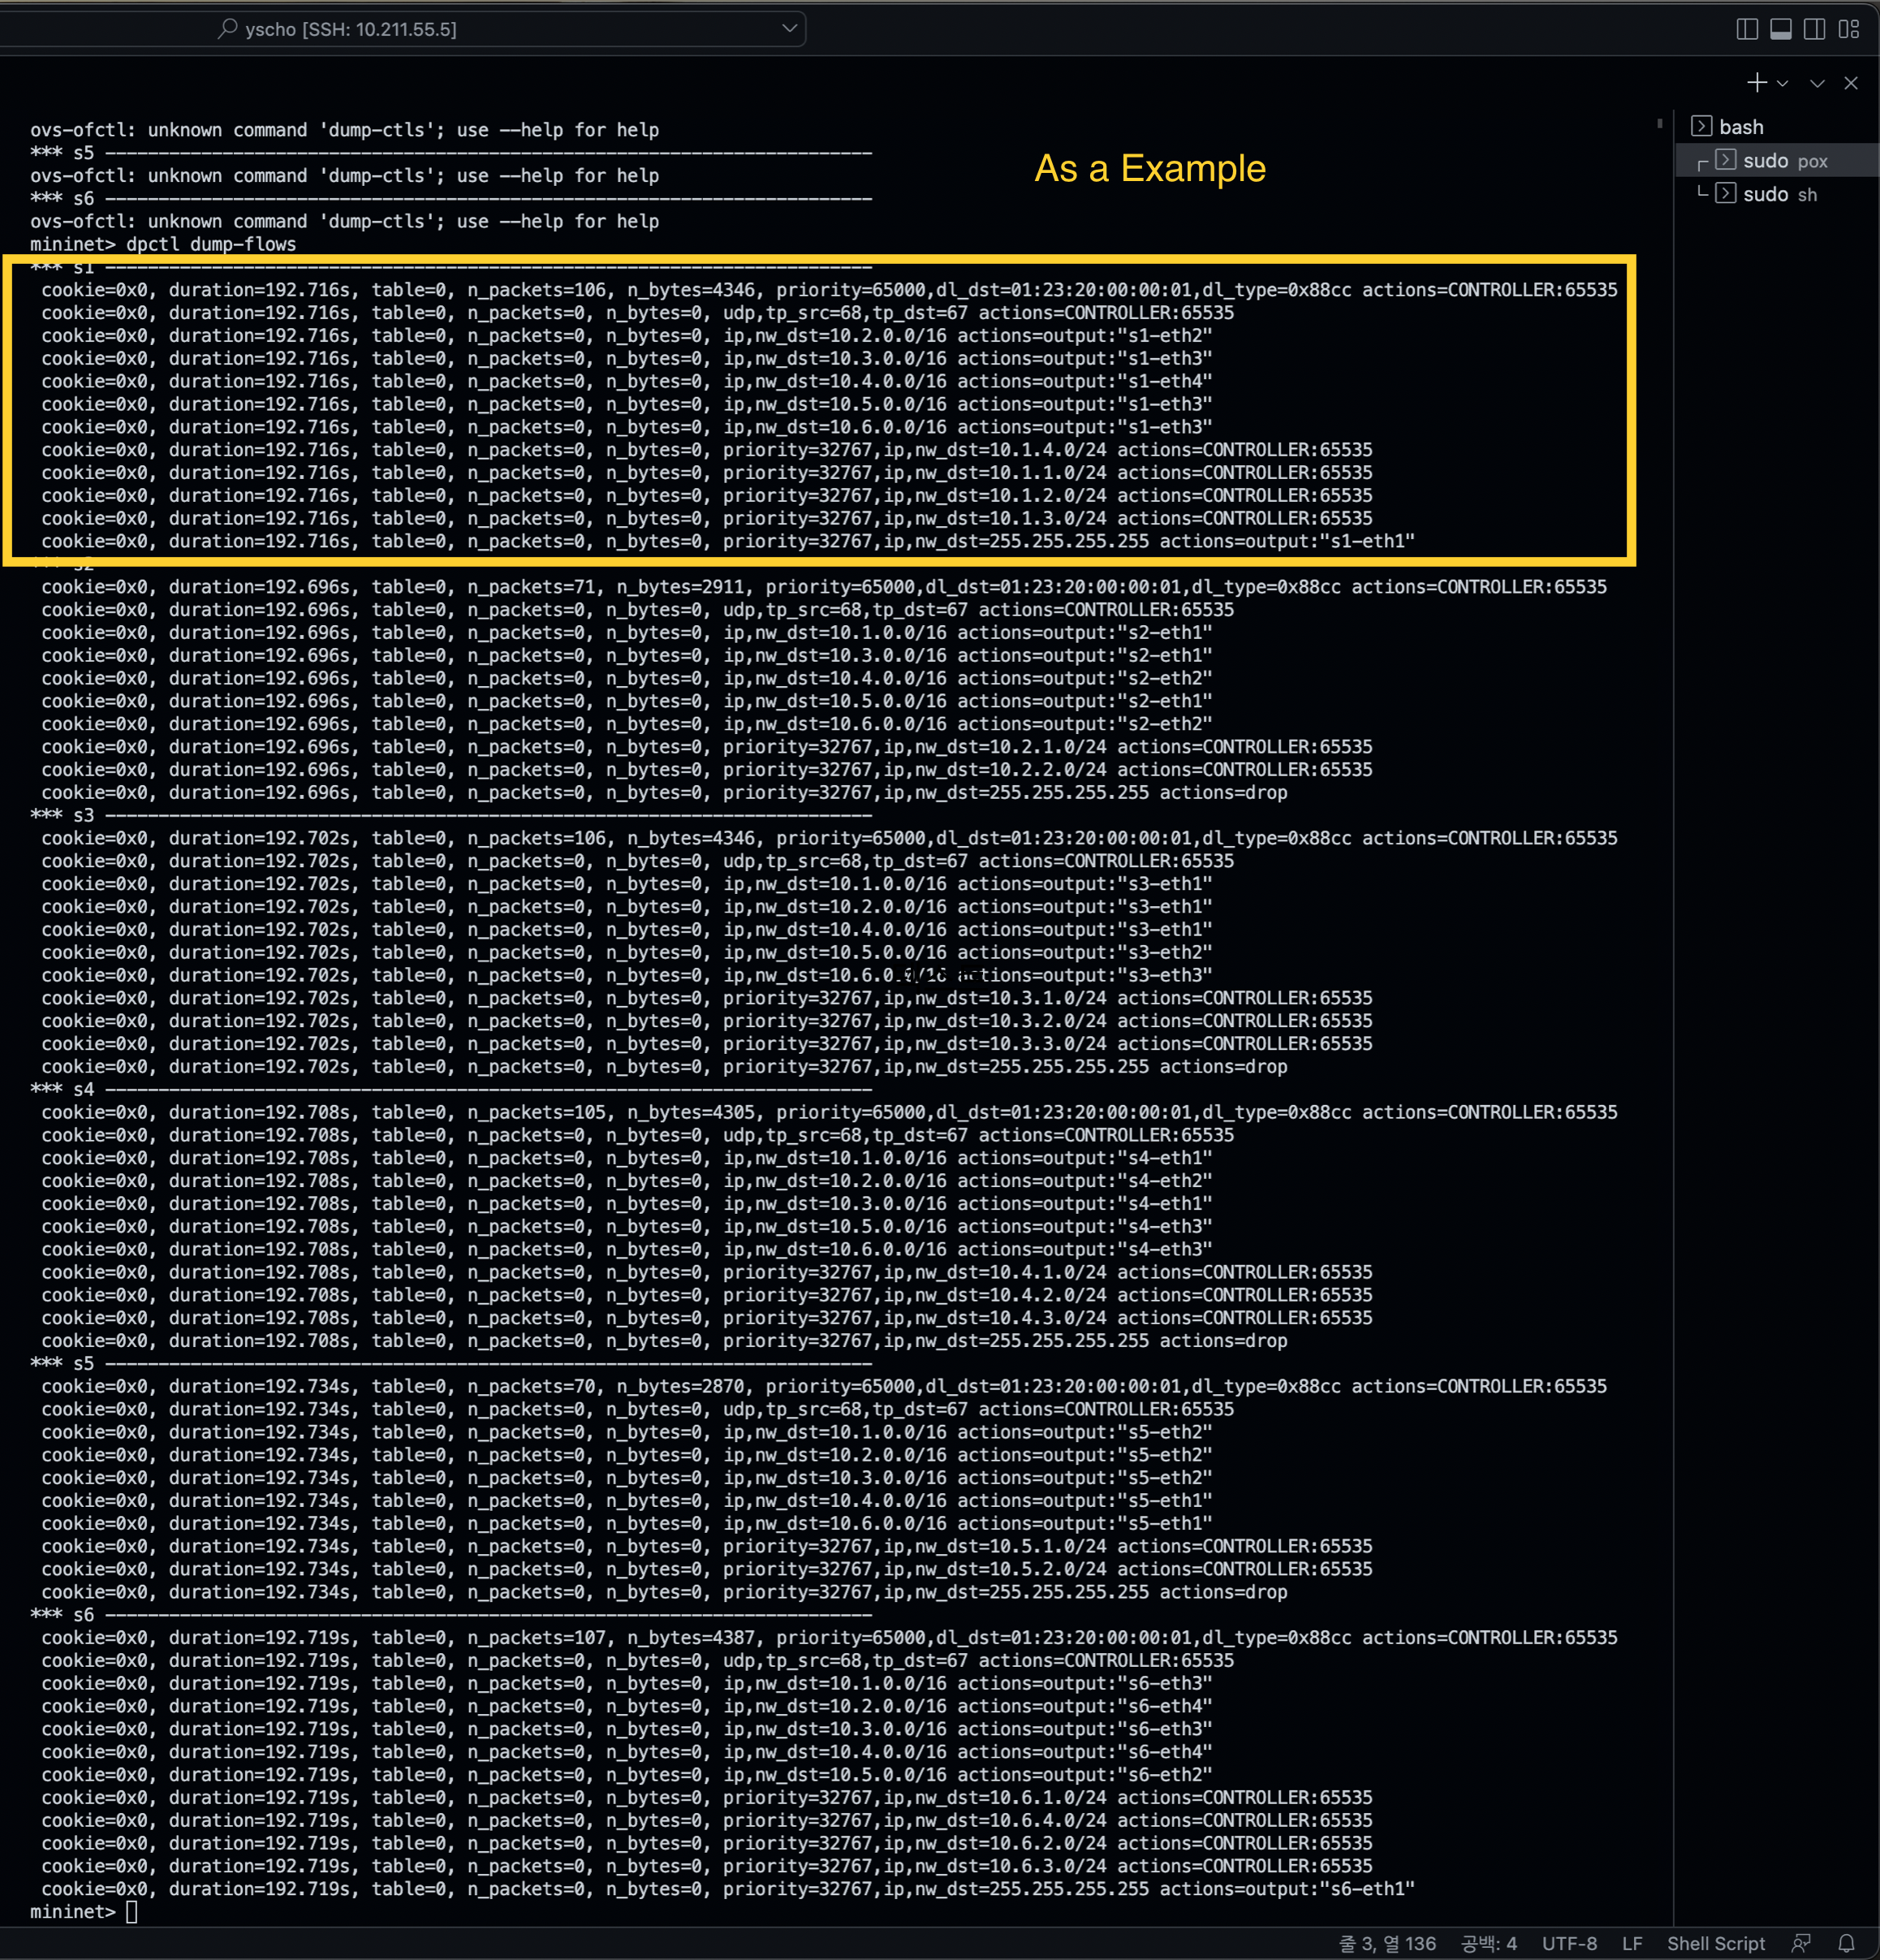
\includegraphics[width=0.5\textwidth]{image/week05/3-1.png}
}
\subfloat[The model graph of custom CNN model (5 layer) ]{
    \includegraphics[width=0.5\textwidth]{image/week05/3-2.png}
}
\caption{The image of the CNN model converted by torchviz }
\end{figure}
\subsection{Test Accuracy Results}
We had 2 experment with custom CNN model with given labeled\_data and custom labeled\_data2.

The test accuracy of the result using the given dataset, "labeled\_data" with custom 5-layer CNN model, we can took the result that the \textbf{Test Accuracy : 89.583}.\\
The test accuracy of the result using the custom dataset, "labeled\_data2" with custom 5-layer CNN model, we can took the result that the \textbf{Test Accuracy : 97.853}.

We can figure out the significant increase of Accuracy campare with the result of Experiment 1 \& 2 that used given 4-layer model. The discussion of the increasement deal with the next bonus section.
\clearpage
    \begin{figure}[!h]\centering 
		\includegraphics[width=.67\textwidth]{image/week05/3-3.png}
		\caption{\footnotesize 
		Terminal out results : Experiment 3-1, given dataset \& custom model \textbf{Test Accuracy : 89.583}}
		\vspace{-10pt}
    \end{figure}
    \begin{figure}[!h]\centering 
		\includegraphics[width=.67\textwidth]{image/week05/4-1.png}
		\caption{\footnotesize 
		Terminal out results : Experiment 3-1, custom dataset \& custom model \textbf{Test Accuracy : 97.853}}
		\vspace{-10pt}
    \end{figure}
\clearpage